% bei Standalone in documentclass noch:
% \RequirePackage{luatex85}

\documentclass[captions=tableheading, titlepage= firstiscover, parskip = half , bibliography=totoc]{scrartcl}
%paper = a5 für andere optinen
% titlepage= firstiscover
% bibliography=totoc für bibdateien
% parskip=half  Veränderung um Absätze zu verbessern

\usepackage{scrhack} % nach \documentclass
\usepackage[aux]{rerunfilecheck}
\usepackage{polyglossia}
\usepackage[style=numeric, backend=biber]{biblatex} % mit [style = alphabetic oder numeric] nach polyglossia
\addbibresource{lit.bib}
\setmainlanguage{german}

\usepackage[autostyle]{csquotes}
\usepackage{amsmath} % unverzichtbare Mathe-Befehle
\usepackage{amssymb} % viele Mathe-Symbole
\usepackage{mathtools} % Erweiterungen für amsmath
\usepackage{fontspec} % nach amssymb
% muss ins document: \usefonttheme{professionalfonts} % für Beamer Präsentationen
\usepackage{longtable}

\usepackage[
math-style=ISO,    % \
bold-style=ISO,    % |
sans-style=italic, % | ISO-Standard folgen
nabla=upright,     % |
partial=upright,   % /
]{unicode-math} % "Does exactly what it says on the tin."
\setmathfont{Latin Modern Math}
% \setmathfont{Tex Gyre Pagella Math} % alternativ

\usepackage[
% die folgenden 3 nur einschalten bei documenten
locale=DE,
separate-uncertainty=true, % Immer Fehler mit ±
per-mode=symbol-or-fraction, % m/s im Text, sonst \frac
]{siunitx}

% alternativ:
% per-mode=reciprocal, % m s^{-1}
% output-decimal-marker=., % . statt , für Dezimalzahlen

\usepackage[
version=4,
math-greek=default,
text-greek=default,
]{mhchem}

\usepackage[section, below]{placeins}
\usepackage{caption} % Captions schöner machen
\usepackage{graphicx}
\usepackage{grffile}
\usepackage{subcaption}

% \usepackage{showframe} Wenn man die Ramen sehen will

\usepackage{float}
\floatplacement{figure}{htbp}
\floatplacement{table}{htbp}

\usepackage{mhchem} %chemische Symbole Beispiel: \ce{^{227}_{90}Th+}


\usepackage{booktabs}

 \usepackage{microtype}
 \usepackage{xfrac}

 \usepackage{expl3}
 \usepackage{xparse}

 % \ExplSyntaxOn
 % \NewDocumentComman \I {}  %Befehl\I definieren, keine Argumente
 % {
 %    \symup{i}              %Ergebnis von \I
 % }
 % \ExplSyntaxOff

 \usepackage{pdflscape}
 \usepackage{mleftright}

 % Mit dem mathtools-Befehl \DeclarePairedDelimiter können Befehle erzeugen werden,
 % die Symbole um Ausdrücke setzen.
 % \DeclarePairedDelimiter{\abs}{\lvert}{\rvert}
 % \DeclarePairedDelimiter{\norm}{\lVert}{\rVert}
 % in Mathe:
 %\abs{x} \abs*{\frac{1}{x}}
 %\norm{\symbf{y}}

 % Für Physik IV und Quantenmechanik
 \DeclarePairedDelimiter{\bra}{\langle}{\rvert}
 \DeclarePairedDelimiter{\ket}{\lvert}{\rangle}
 % <name> <#arguments> <left> <right> <body>
 \DeclarePairedDelimiterX{\braket}[2]{\langle}{\rangle}{
 #1 \delimsize| #2
 }

\setlength{\delimitershortfall}{-1sp}

 \usepackage{tikz}
 \usepackage{tikz-feynman}

 \usepackage{csvsimple}
 % Tabellen mit \csvautobooktabular{"file"}
 % muss in table umgebung gesetzt werden


% \multicolumn{#Spalten}{Ausrichtung}{Inhalt}

\usepackage{hyperref}
\usepackage{bookmark}
\usepackage[shortcuts]{extdash} %nach hyperref, bookmark

\newcommand{\ua}[1]{_\symup{#1}}
\newcommand{\su}[1]{\symup{#1}}


\begin{document}

\section{Messwerte}

\begin{table}
  \centering
  \caption{gemessene Werte}
  \label{tab:Messdaten}
  \begin{tabular}{c c c c c }
    \toprule $Fallzeit \,\, Kugel \, 2 \,\, [\symup{s}]$ & $Fallzeit\,\, Kugel\, 1 \,\, [\symup{s}]$ & $Temperatur \,\, [\symup{°C}]$ & $Messung \, 1 \,\, [\symup{s}]$ & $Messung \, 2 \,\, [\symup{s}]$ \\
    \midrule
    11.80 & 68.47 & 31.0 & 68.86 & 68.86 \\
    11.80 & 68.95 & 36.0 & 68.33 & 68.21 \\
    12.15 & 68.69 & 39.0 & 65.75 & 65.76 \\
    11.73 & 68.53 & 45.0 & 60.32 & 60.52 \\
    12.21 & 68.50 & 49.5 & 59.27 & 59.27 \\
    11.47 & 67.69 & 51.5 & 58.52 & 58.66 \\
    12.10 & 68.83 & 56.0 & 58.30 & 58.29 \\
    11.96 & 68.41 & 60.0 & 56.60 & 56.72 \\
    11.86 & 68.38 & 64.0 & 55.10 & 55.15 \\
    11.87 & 68.60 & 68.0 & 54.35 & 54.40 \\
    \bottomrule
  \end{tabular}
\end{table}

\begin{table}
  \centering
  \caption{Mittelwerte der Fallzeiten \texorpdfstring{$[\symup{s}]$}{b} für Teil 1 des Versuches}
  \begin{tabular}{c c c c}
    \toprule $Fallzeit \,\, Kugel \,\, 1$ & $\increment_{FK1}$ & $Fallzeit \,\, Kugel \,\, 2$ & $\increment_{FK2}$ \\
    \midrule
    68.50 & 0.30 & 11.89 & 0.13 \\
    \bottomrule
  \end{tabular}
  \label{tab:FallzeitenGemittelt}
\end{table}

\begin{table}
  \centering
  \caption{Mittelwerte der Messung bei verschiedenen Temperaturen für die große Kugel}
  \label{tab:TemperaturGemittelt}
  \begin{tabular}{c | c c c c c c c c c c }
    \toprule
    $Temperatur \,\, [\symup{K}]$          & 304.15 & 309.15 & 312.15 & 318.15 & 322.65 \\
    $Fallzeit \,\, [\symup{s}]$            & 68.86 & 68.27 & 65.76 & 60.42 & 59.27 \\
    $\increment_{FZ} \,\, [\symup{s}]$     & 0 & 0.035 & 0.002 & 0.058 & 0 \\
    \midrule
    $Temperatur \,\, [\symup{K}]$          & 324.65 & 329.15 & 333.15 & 337.15 & 341.15 \\
    $Fallzeit \,\, [\symup{s}]$            & 58.59 & 58.29 & 56.66 & 55.13 & 54.38 \\
    $\increment_{FZ} \,\, [\symup{s}]$     & 0.040 & 0.003 & 0.035 & 0.014 & 0.014 \\
    \bottomrule
  \end{tabular}
\end{table}

\newpage

\section{Auswertung}

\subsection{Bestimmung der Apparatekonstante für die große Kugel}

In dem ersten Teil des Versuches soll die Apparatekonstante für die große Kugel (Kugel 1) bestimmt
werden. Dafür wird mithilfe der bekannten Apparatekonstante für die kleine Kugel (Kugel 2) die Viskosität
des Wassers bei Raumtemperatur bstimmt und in folgende Formel eingesetzt:

\begin{align}
  \label{eqn:KappaGroß}
  \Kappa_{kl} &= 0.007640 \, \symup{[mPa\, cm^3 / g]} \\
  \eta        &= \Kappa_{gr} \cdot \left( \rho_K - \rho_{Fl} \right) \cdot t
\end{align}

Bei $\rho_K$ und $\rho_{Fl}$ handelt es sich um die Dichten der Kugel und der betrachteten
Flüssigkeit. Mithilfe der gemessenen Radien und Gewichte der Kugeln kann die Dichte
bestimmt werden:

\begin{align}
  r_{gr}    &= (0.0078017 \pm 0.0000017) \, \symup{[m]}     & r_{kl}    &= (0.0077167 \pm 0.0000017) \, \symup{[m]} \\
  m_{gr}    &= 0.00496 \, \symup{[kg]}                        & m_{kl}    &= 0.00446 \, \symup{[kg]} \\
  \rho_{gr} &= (2493.6 \pm 1.6) \, \symup{\left[ kg/m^3\right]} & \rho_{gr} &= (2312.0 \pm 1.5) \, \symup{\left[ kg/m^3\right]}
\end{align}

In Tabelle \ref{tab:FallzeitenGemittelt} sind die Mittelwerte und Fehler der gemessenen Fallzeiten für die
kleine und Große Kugel bei Raumtemperatur eingetragen.
Somit ergeben sich für die Viskosität des Wassers bei Raumtemperatur $\eta_{20}$ und $K_{gr}$ folgende Werte:

\begin{align}
  \eta_{20}   &= (0.001194 \pm 0.00013) \, \symup{[Pa \, s]} \\
  \Kappa_{gr} &= \frac{\eta_{20}}{\left( \rho_{gr} - \rho_{w} \right) \cdot t_{gr}} \\
              &= (0.001165 \pm, 0.00012) \, \symup{[mPa\, cm^3 / g]}
\end{align}

Die Fehler für $\eta_{20}$ und $\Kappa_{gr}$ ergeben sich mit der Gaußschen Fehlerfortpflanzung:

\begin{align}
\increment \eta    &= \sqrt{ \left( \partial_{\rho_{gr}} \eta \cdot \increment \rho_{gr} \right)^2 + \left( \partial_{t_{gr}} \eta \cdot \increment t_{gr} \right)^2  }\\
\increment K_{gr} &= \sqrt{ \left( \partial_{\eta} K_{gr} \cdot \increment \eta \right)^2 + \left( \partial_{\rho_{gr}} K_{gr} \cdot \increment \rho_{gr} \right)^2 +
                      \left( \partial_{t_{gr}} K_{gr} \cdot \increment t_{gr} \right)^2  }
\end{align}

\begin{figure}
  \centering
  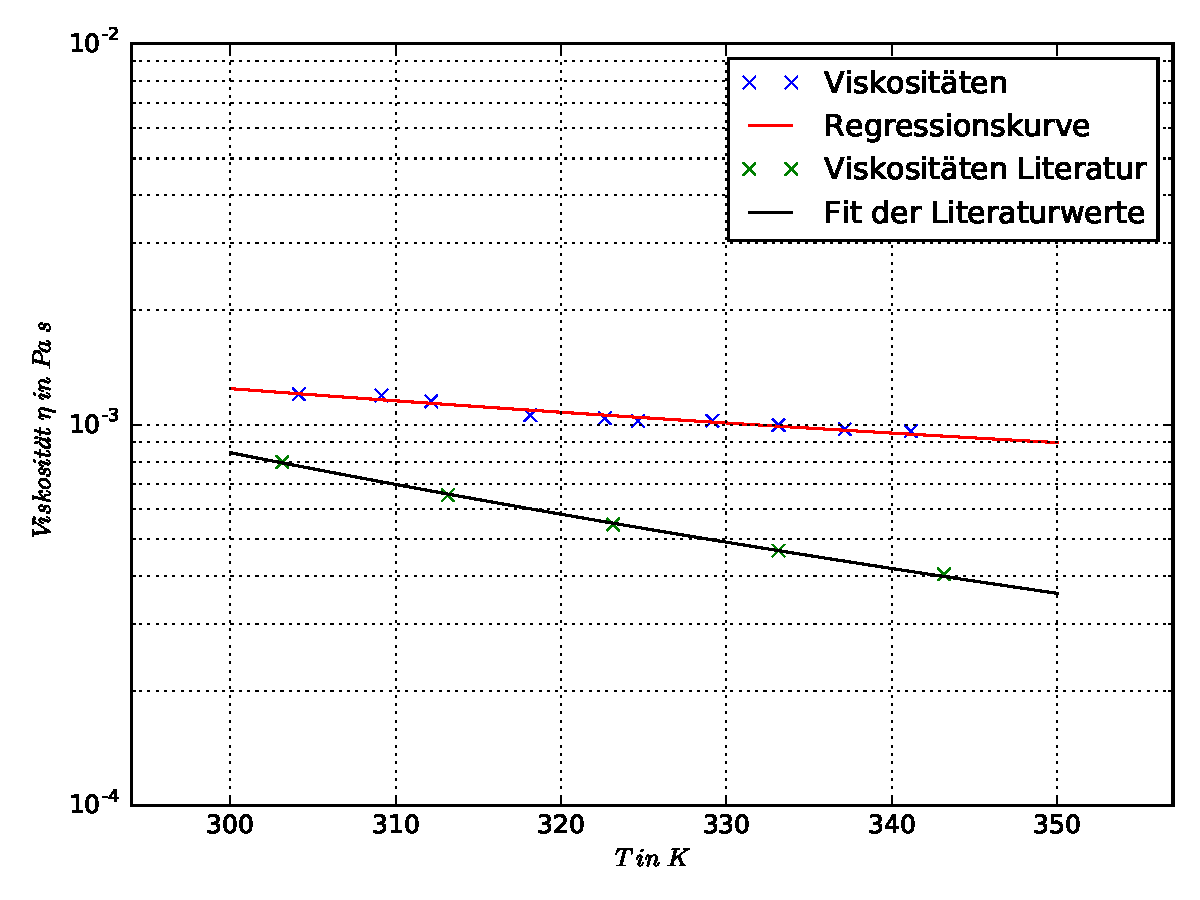
\includegraphics[height = 9 cm]{Plot_T.pdf}
  \caption{Viskositäten gegen T}
  \label{plt:ViskosT}
\end{figure}

\begin{figure}
  \centering
  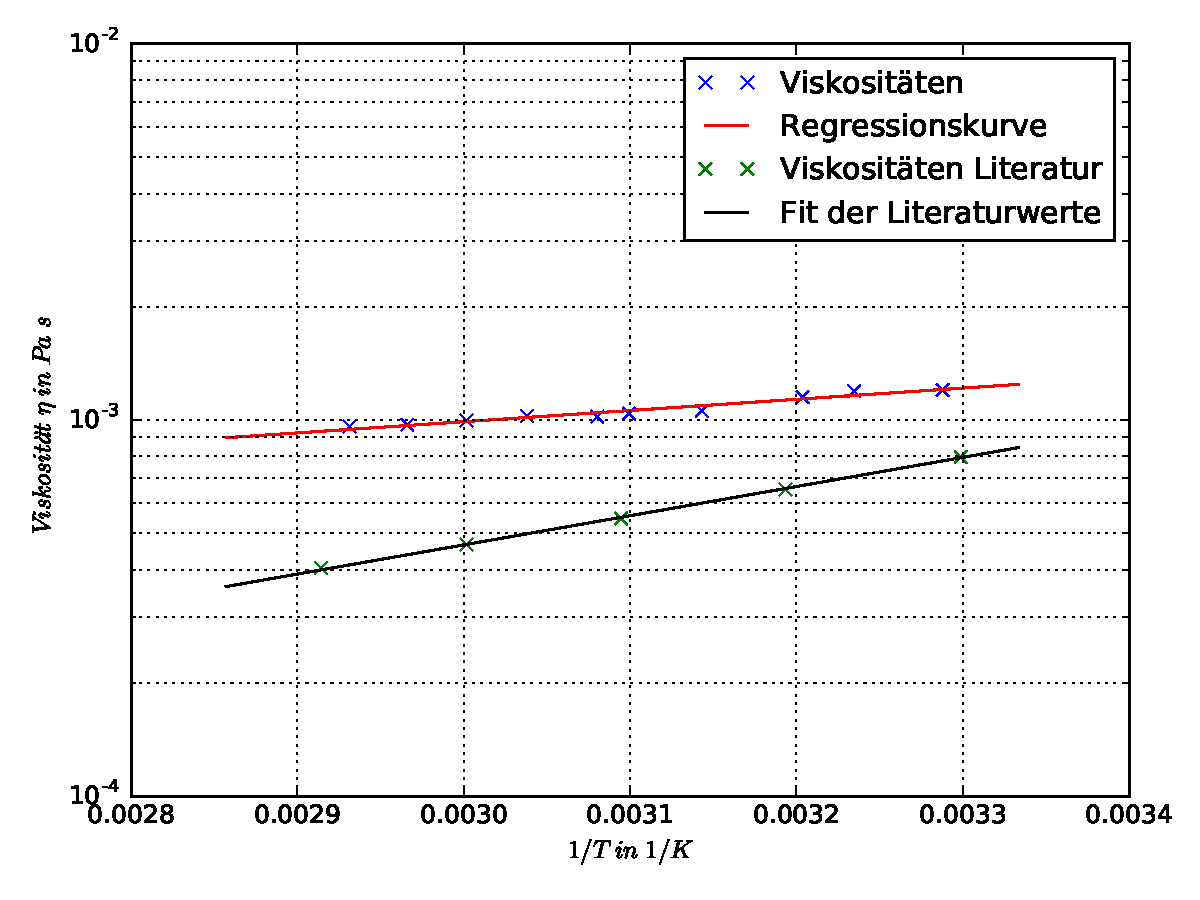
\includegraphics[height = 9 cm]{Plot_T_1.pdf}
  \caption{Viskositäten gegen 1/T}
  \label{plt:Viskos_T}
\end{figure}

\subsection{Bestimmung der Konstanten A/B für die zeitabhängige Viskosität \texorpdfstring{$\eta(T)$}{z}}

In den beiden Abbildungen \ref{plt:ViskosT} und \ref{plt:Viskos_T} sieht man einmal die Viskosität gegen T und einmal gegen 1/T aufgetragen.
Zum Vergleich sind in beiden Graphen auch die Literaturwerte mit eingebunden.
Die y - Skala ist dabei logarythmisch angepasst. Die Plots wurden mithilfe von Python erstellt und ergeben
für A und B folgende Parameter:

\begin{align}
  \symup{A} &= 1.2651 \cdot 10^{-4} \\
  \symup{B} &= 6.8567 \cdot 10^{2}
\end{align}

Somit ergibt sich für die Andradesche Gleichung für die Temperaturabhängigkeit der Viskosität von destilliertem
Wasser folgende Formel:

\begin{equation}
  \eta(\symup{T}) = 1.2651 \cdot 10^{-4} \cdot \exp \left( \frac{6.8567 \cdot 10^{2}}{\symup{T}} \right)
\end{equation}

\subsection{Bestimmung der Reynoldszahl}

Mithilfe der folgenden Formel für die Reynoldszahl kann bei dem vorliegenden Versuch beurteilt werden, ob es
sich um eine laminare Strömung handelt.

\begin{equation}
  R = \frac{ \rho_{w} \cdot v \cdot d}{\eta}
\end{equation}


Als kritische Zahl für Rohrströmungen gilt normalerweise ein Faktor von ca. 2300. Da für das $d$ in diesem
Fall jedoch nicht der Querschnitt der Strömung, sondern der Durchmesser der umströmten Kugel verwendet wird,
halbiert sich dieser Wert zu $R_{krit} = 1150$.

Die Geschwindigkeit der Kugel für die verschiedenen Temperaturen lassen sich mit den gemessenen Fallzeiten in
Tabelle \ref{tab:TemperaturGemittelt} und der vorher bekannten Messtrecke von $S = 0.1$ m berechnen. Sie sind
in der folgenden Tabelle eingetragen.

\begin{table}
  \centering
  \caption{Geschwindigkeit der großen Kugel für verschiedene Geschwindigkeiten}
  \label{tab:Geschwindigkeiten}
  \begin{tabular}{c | c c c c c }
    \toprule
    $v \,\, in \,\, \left[ \frac{m}{s} \right]$ & 0.145 & 0.146 & 0.152 & 0.166 & 0.169 \\
    $\increment v \,\, in \,\, \left[ \frac{m}{s} \cdot 10^{-5} \right]$ & $0$ & $7.432$ & $0.667$ & $15.81$ & $0$ \\
    \midrule
    $v \,\, in \,\, \left[ \frac{m}{s} \right]$ & 0.171 & 0.172 & 0.176 & 0.181 & 0.184 \\
    $\increment v \,\, in \,\, \left[ \frac{m}{s} \cdot 10^{-5} \right ]$ & $11.77$ & $0.849$ & $10.79$ & $4.749$ & $4.882$ \\
    \bottomrule
  \end{tabular}
\end{table}





\end{document}
